\begin{center}

\includegraphics[width=0.4\textwidth]{content/3/chapter4/images/41.png}\\
Cippi滑下滑梯
\end{center}

C++20中,Lambda表达式支持模板参数和概念,可以有默认构造,并在没有状态时支持复制赋值。此外,Lambda表达式可以在未计算的上下文中使用,还会检测何时隐式复制this指针。

先从Lambda的模板参数开始吧。

\subsubsubsection{4.7.1\hspace{0.2cm}Lambda的模板参数}

C++20中类型化Lambda(C++11)、泛型Lambda(C++14)和模板Lambda(Lambda的模板形参)之间的差异很小。

\begin{lstlisting}[style=styleCXX]
// templateLambda.cpp

#include <iostream>
#include <string>
#include <vector>

auto sumInt = [](int fir, int sec) { return fir + sec; };
auto sumGen = [](auto fir, auto sec) { return fir + sec; };
auto sumDec = [](auto fir, decltype(fir) sec) { return fir + sec; };
auto sumTem = []<typename T>(T fir, T sec) { return fir + sec; };

 int main() {
	
	 std::cout << '\n';
	
	 std::cout << "sumInt(2000, 11): " << sumInt(2000, 11) << '\n';
	 std::cout << "sumGen(2000, 11): " << sumGen(2000, 11) << '\n';
	 std::cout << "sumDec(2000, 11): " << sumDec(2000, 11) << '\n';
	 std::cout << "sumTem(2000, 11): " << sumTem(2000, 11) << '\n';
	
	 std::cout << '\n';
	
	 std::string hello = "Hello ";
	 std::string world = "world";
	 // std::cout << "sumInt(hello, world): " << sumInt(hello, world) << '\n';
	 std::cout << "sumGen(hello, world): " << sumGen(hello, world) << '\n';
	 std::cout << "sumDec(hello, world): " << sumDec(hello, world) << '\n';
	 std::cout << "sumTem(hello, world): " << sumTem(hello, world) << '\n';
	
	
	 std::cout << '\n';
	
	 std::cout << "sumInt(true, 2010): " << sumInt(true, 2010) << '\n';
	 std::cout << "sumGen(true, 2010): " << sumGen(true, 2010) << '\n';
	 std::cout << "sumDec(true, 2010): " << sumDec(true, 2010) << '\n';
	 // std::cout << "sumTem(true, 2010): " << sumTem(true, 2010) << '\n';
	
	 std::cout << '\n';
	
}
\end{lstlisting}

在展示程序输出之前,我想比较一下这四个Lambda表达式。

\begin{itemize}
\item 
sumInt
\begin{itemize}
\item 
C++11

\item 
类型化Lambda

\item 
只接受能转换为int的类型
\end{itemize}

\item 
sumGen
\begin{itemize}
\item 
C++14

\item 
泛型Lambda

\item 
可接受所有类型
\end{itemize}

\item 
sumDec
\begin{itemize}
\item 
C++14

\item 
泛型Lambda

\item 
第二个参数的类型必须可以转换为第一个参数的类型
\end{itemize}

\item 
sumTem
\begin{itemize}
\item 
C++20

\item 
模板Lambda

\item 
两个参数类型必须相同
\end{itemize}
\end{itemize}

这对于不同类型的模板参数意味着什么?当然,每个Lambda传入的都是int型变量(第16-19行),而类型化的Lambda sumInt不接受字符串(第25行)。

将bool true和int 2010传递给Lambda可能会有出乎意料(第33-36行)的结果。

\begin{itemize}
\item 
sumInt返回2011,true可以是一个整型值,可升格为int。

\item 
sumGen返回2011,true可以是一个整型值,可升格为int。sumInt和sumGen之间有一个细微的区别。

\item 
sumDec返回2。为什么?第二个形参sec的类型变成了第一个形参fir的类型:因为decltype(fir) sec,编译器推导出了fir的类型,其类型与sec类型相同。因此,2010转换为true。在表达式fir + sec中,fir提升为1,所以结果是2。

\item 
sumTem是无效的。
\end{itemize}

\begin{tcblisting}{commandshell={}}
sumInt(2000, 11): 2011
sumGen(2000, 11): 2011
sumDec(2000, 11): 2011
sumTem(2000, 11): 2011

sumGen(hello, world): Hello world
sumDec(hello, world): Hello world
sumTem(hello, world): Hello world

sumInt(true, 2010): 2011
sumGen(true, 2010): 2011
sumDec(true, 2010): 2
\end{tcblisting}

模板Lambda的典型的用例是在Lambda中使用容器。下面的代码给出了三个接受容器的Lambda表达式,每个表达式都会返回容器的大小。

\hspace*{\fill} \\ %插入空行
\noindent
\textbf{三个Lambda表达式都可以接受容器}
\begin{lstlisting}[style=styleCXX]
// templateLambdaVector.cpp

#include <concepts>
#include <deque>
#include <iostream>
#include <string>
#include <vector>

auto lambdaGeneric = [](const auto& container) { return container.size(); };
auto lambdaVector = []<typename T>(const std::vector<T>& vec) { return vec.size(); };
auto lambdaVectorIntegral = []<std::integral T>(const std::vector<T>& vec) {
	return vec.size();
};

 int main() {
	
	
	std::cout << '\n';
	
	std::deque deq{1, 2, 3};
	std::vector vecDouble{1.1, 2.2, 3.3, 4.4};
	std::vector vecInt{1, 2, 3, 4, 5};
	
	std::cout << "lambdaGeneric(deq): " << lambdaGeneric(deq) << '\n';
	// std::cout << "lambdaVector(deq): " << lambdaVector(deq) << '\n';
	// std::cout << "lambdaVectorIntegral(deq): "
	// << lambdaVectorIntegral(deq) << '\n';
	
	std::cout << '\n';
	
	std::cout << "lambdaGeneric(vecDouble): " << lambdaGeneric(vecDouble) << '\n';
	std::cout << "lambdaVector(vecDouble): " << lambdaVector(vecDouble) << '\n';
	// std::cout << "lambdaVectorIntegral(vecDouble): "
	// << lambdaVectorIntegral(vecDouble) << '\n';
	
	std::cout << '\n';
	
	std::cout << "lambdaGeneric(vecInt): " << lambdaGeneric(vecInt) << '\n';
	std::cout << "lambdaVector(vecInt): " << lambdaVector(vecInt) << '\n';
	std::cout << "lambdaVectorIntegral(vecInt): "
	<< lambdaVectorIntegral(vecInt) << '\n';
	
	std::cout << '\n';
	
	}
\end{lstlisting}

函数lambdaGeneric(第9行)可以接受有成员函数size()的数据类型。函数lambdaVector(第10行)更具体:只接受std::vector。函数lambdaVectorIntegral(第11行)使用C++20概念std::integral,所以只接受使用整型(如int)的std::vector。为了使用std::integral概念,必须包含头文件<concepts>。

\begin{tcblisting}{commandshell={}}
lambdaGeneric(deq): 3

lambdaGeneric(vecDouble): 4
lambdaVector(vecDouble): 4

lambdaGeneric(vecInt): 5
lambdaVector(vecInt): 5
lambdaVectorIntegral(vecInt): 5
\end{tcblisting}

\begin{tcolorbox}[breakable,enhanced jigsaw,colback=mygreen!5!white,colframe=mygreen!75!black,title={类模板参数的推导}]
templateLambdaVector.cpp中有个可能会错过的特性。从C++17开始,编译器就可以从类模板的实参推断类模板的类型(第20-22行)。初始化vector时,可以这样写std::vector myVec{1,2,3},而非冗长的std::vector<int> myVec{1,2,3}。
\end{tcolorbox}

\subsubsubsection{4.7.2\hspace{0.2cm}检测并隐式复制this指针}

C++20编译器会检测何时隐式复制this指针。复制隐式捕获的this指针会导致未定义的行为,例如:

\begin{lstlisting}[style=styleCXX]
// lambdaCaptureThis.cpp

#include <iostream>
#include <string>

struct LambdaFactory {
	auto foo() const {
		return [=] { std::cout << s << '\n'; };
	}
	std::string s = "LambdaFactory";
	~LambdaFactory() {
		std::cout << "Goodbye" << '\n';
	}
};

auto makeLambda() {
	LambdaFactory lambdaFactory; 
	
	return lambdaFactory.foo();
}


int main() {

	std::cout << '\n';
	
	auto lam = makeLambda();
	lam();
	
	std::cout << '\n';

}
\end{lstlisting}

程序的编译没问题,但这并不说明程序执行起来没问题。

\begin{center}
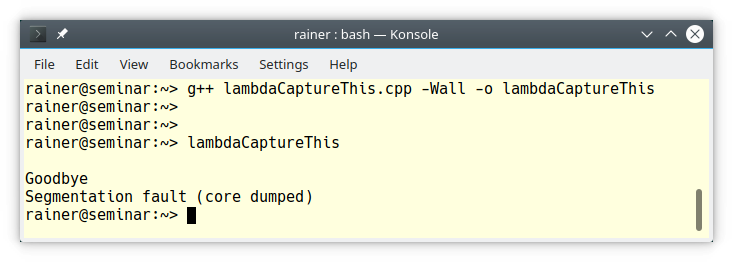
\includegraphics[width=0.8\textwidth]{content/3/chapter4/images/42.png}\\
由于未定义行为造成的段错误
\end{center}

发现lambdaCaptureThis.cpp中的问题了吗?成员函数foo(第7行)返回表达式 [=] {std::cout <{}< s <{}< '\verb|\|n';}具有this指针的隐式副本。这个隐式复制在(第17行)中没有问题,但是在作用域的末尾就成了问题。作用域的结束意味着局部Lambda生命周期的结束(第19行),所以使用lam()(第28行)会触发未定义的行为。

这种情况下,C++20编译器会发出警告。

\begin{center}
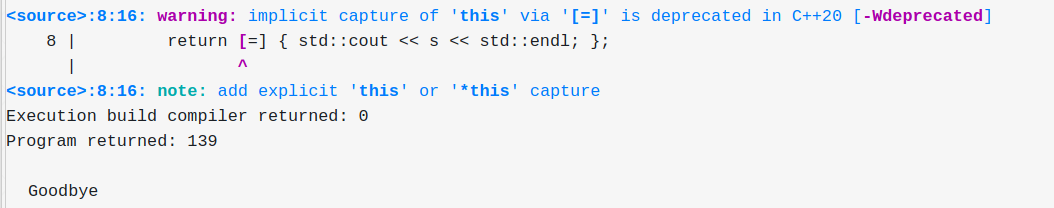
\includegraphics[width=1.0\textwidth]{content/3/chapter4/images/1-8.png}\\
\end{center}

C++20的最后两个Lambda特性结合起来非常好用:C++20中的Lambda可以使用默认构造,并且在没有状态时支持复制赋值。此外,Lambda表达式可以在未计算的上下文中使用。

\subsubsubsection{4.7.3\hspace{0.2cm}未计算上下文中的Lambda和无状态的Lambda可以默认构造和复制赋值}

本节的标题包含两个术语:未计算的上下文和无状态的Lambda。先从“未计算的上下文”开始说起。

\hspace*{\fill} \\ %插入空行
\noindent
\textbf{4.7.3.1\hspace{0.2cm}未计算的上下文}

下面的代码段具有函数声明和函数定义。

\begin{lstlisting}[style=styleCXX]
int add1(int, int); // declaration
int add2(int a, int b) { return a + b; } // definition
\end{lstlisting}

函数add1是声明的,而add2是定义。若在已计算的上下文中使用add1,例如:通过调用将得到一个链接时错误。关键是可以在未计算的上下文中使用add1,例如\href{https://en.cppreference.com/w/cpp/language/typeid}{typeid}或\href{https://en.cppreference.com/w/cpp/language/decltype}{decltype},两个操作符都接受未计算的操作数。

\begin{lstlisting}[style=styleCXX]
// unevaluatedContext.cpp

#include <iostream>
#include <typeinfo> // typeid

int add1(int, int); // declaration
int add2(int a, int b) { return a + b; } // definition

int main() {
	
	std::cout << '\n';
	
	std::cout << "typeid(add1).name(): " << typeid(add1).name() << '\n';
	
	decltype(*add1) add = add2;
	
	std::cout << "add(2000, 20): " << add(2000, 20) << '\n';
	
	std::cout << '\n';

}
\end{lstlisting}

typeid(add1).name()(第13行)返回类型的字符串表示形式,decltype(第15行)可以推导其参数的类型。

\begin{center}
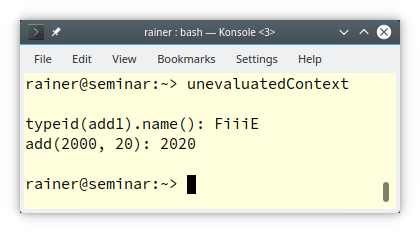
\includegraphics[width=0.6\textwidth]{content/3/chapter4/images/43.png}\\
\end{center}

\hspace*{\fill} \\ %插入空行
\noindent
\textbf{4.7.3.2\hspace{0.2cm}无状态的Lambda}

无状态是指不捕获任何内容的Lambda。换句话说,无状态的Lambda是定义中初始中括号[]为空的Lambda。例如,Lambda表达式auto add = [](int a, int b) \{return a + b;\};就是无状态的。

\hspace*{\fill} \\ %插入空行
\noindent
\textbf{4.7.3.3\hspace{0.2cm}适配标准模板库中的关联容器}

展示示例之前,先添加一些注释。容器std::set和其他来自标准模板库的有序关联容器(std::map, std::multiset和std::multimap)默认使用函数对象std::less对键进行排序。std::less按字典升序对所有键进行排序。\href{https://en.cppreference.com/w/cpp/container/set}{std::set}的声明,隐式使用了std::less。

\hspace*{\fill} \\ %插入空行
\noindent
\textbf{std::set的声明}
\begin{lstlisting}[style=styleCXX]
template<
	class Key,
	class Compare = std::less<Key>,
	class Allocator = std::allocator<Key>
> class set;
\end{lstlisting}

再来看看排序。

\hspace*{\fill} \\ %插入空行
\noindent
\textbf{Lambda用于未计算的上下文中}
\begin{lstlisting}[style=styleCXX]
// lambdaUnevaluatedContext.cpp

#include <cmath>
#include <iostream>
#include <memory>
#include <set>
#include <string>

template <typename Cont>
void printContainer(const Cont& cont) {
	for (const auto& c: cont) std::cout << c << " ";
	std::cout << "\n";
}

 int main() {
	
	std::cout << '\n';
	
	std::set<std::string> set1 = {"scott", "Bjarne", "Herb", "Dave", "michael"};
	printContainer(set1);
	
	using SetDecreasing = std::set<std::string,
									decltype([](const auto& l, const auto& r) {
	 									return l > r;
									})>;
	SetDecreasing set2 = {"scott", "Bjarne", "Herb", "Dave", "michael"};
	printContainer(set2);
	
	using SetLength = std::set<std::string,
							decltype([](const auto& l, const auto& r) {
	 							return l.size() < r.size();
							})>;
	SetLength set3 = {"scott", "Bjarne", "Herb", "Dave", "michael"};
	printContainer(set3);
	
	std::cout << '\n';
	
	std::set<int> set4 = {-10, 5, 3, 100, 0, -25};
	printContainer(set4);
	
	using setAbsolute = std::set<int, decltype([](const auto& l, const auto& r) {
	 												return std::abs(l)< std::abs(r);
	})>;
	setAbsolute set5 = {-10, 5, 3, 100, 0, -25};
	printContainer(set5);
	
	std::cout << "\n\n";

}
\end{lstlisting}

set1(第19行)和set4(第38行)按升序排序键。set2(第26行)、set3(第33行)和set5(第44行)都以相同的方式对其键进行排序,在未计算的上下文中使用Lambda。使用using关键字(第22行)声明了一个类型别名,下一行(第26行)中使用它来定义set。创建std::set会使用无状态Lambda表达式的默认构造函数。

下面是程序的输出。

\begin{tcblisting}{commandshell={}}
Bjarne Dave Herb michael scott
scott michael Herb Dave Bjarne
Herb scott Bjarne michael

-25 -10 0 3 5 100
0 3 5 -10 -25 100
\end{tcblisting}

在研究该程序的输出时,可能会感到惊讶。set3有些特殊,使用[](const auto\& l, const auto\& r)\{return l.size() < r.size();\}作为谓词,并且忽略了Dave。因为Dave和Herb字符串的长度一样,而Herb是先添加的,所以忽略Dave。std::set支持唯一键,所以使用特殊谓词的键相同。若使用std::multiset,这就不会发生这种情况。

\begin{tcolorbox}[breakable,enhanced jigsaw,colback=mygreen!5!white,colframe=mygreen!75!black,title={总结}]
C++20中,Lambda表达式可以有模板参数。此外,Lambda会检测this指针何时隐式引用。
\end{tcolorbox}

\newpage








